\documentclass{article}
\usepackage{amsmath, amssymb, amscd, amsthm, amsfonts}
\usepackage{graphicx}
\usepackage{hyperref}
\usepackage{xcolor}
\usepackage{braket}
\usepackage{cancel}
\usepackage{float}

\oddsidemargin 0pt
\evensidemargin 0pt
\marginparwidth 40pt
\marginparsep 10pt
\topmargin -20pt
\headsep 10pt
\textheight 8.7in
\textwidth 6.65in
\linespread{1.2}

\title{PHYS401: Quantum Mechanics I \\ Homework \#11}
\author{Evan Shipley-Friedt}
\date{December 10th, 2025}

% Extra spacing around equations
\setlength{\abovedisplayskip}{18pt}
\setlength{\belowdisplayskip}{18pt}
\setlength{\abovedisplayshortskip}{14pt}
\setlength{\belowdisplayshortskip}{14pt}

\begin{document}

\maketitle

{\huge Problem 1: Hydrogen atom - Probability for $r<a_0$}

\section*{Solution}

For a separated eigenstate
\[
\psi_{n\ell m}(r,\theta,\phi)=R_{n\ell}(r)\,Y_\ell^m(\theta,\phi),
\]
the probability of finding the electron within radius $a_0$ is
\[
P(r<a_0)=\int_{r<a_0}|\psi|^2\,d^3r
=\int_0^{a_0} r^2 |R_{n\ell}(r)|^2\,dr \int |Y_\ell^m|^2\,d\Omega.
\]
Because the angular eigenfunctions are normalized on the unit sphere,
\[
\int |Y_\ell^m|^2\,d\Omega=1,
\]
then radial-only result is
\[
\boxed{
P_{n\ell}(r<a_0)=\int_0^{a_0} r^2 |R_{n\ell}(r)|^2\,dr
}
\]

%------------------------------------------------------------

\subsection*{$2s$ state: $(n,\ell)=(2,0)$}

From Table 8.1,
\[
R_{20}(r)=2\left(\frac{Z}{2a_0}\right)^{3/2}\left(1-\frac{Zr}{2a_0}\right)e^{-Zr/2a_0}
\]
For hydrogen ($Z=1$),
\[
R_{20}(r)=2\left(\frac{1}{2a_0}\right)^{3/2}\left(1-\frac{r}{2a_0}\right)e^{-r/2a_0}
\]
Then
\[
P_{2s}(r<a_0)=\int_0^{a_0} r^2 |R_{20}(r)|^2\,dr
\]
Let $\rho=r/a_0$ ($0\le\rho\le 1$), so $r=a_0\rho$ and $dr=a_0\,d\rho$.  Also,
\[
|R_{20}(r)|^2
=4\left(\frac{1}{2a_0}\right)^3\left(1-\frac{\rho}{2}\right)^2e^{-\rho}
=\frac{1}{2a_0^3}\left(1-\frac{\rho}{2}\right)^2e^{-\rho}
\]
Therefore
\[
P_{2s}(r<a_0)=\int_0^1 \left(a_0^2\rho^2\right)\left[\frac{1}{2a_0^3}\left(1-\frac{\rho}{2}\right)^2e^{-\rho}\right]\left(a_0\,d\rho\right)
=\frac{1}{2}\int_0^1 \rho^2\left(1-\frac{\rho}{2}\right)^2 e^{-\rho}\,d\rho
\]
Evaluating the integral,
\[
\boxed{
P_{2s}(r<a_0)=1-\frac{21}{8e}\approx 3.43\times 10^{-2}
}
\]

%------------------------------------------------------------

\subsection*{$2p$ states: $(n,\ell)=(2,1)$ with $m=-1,0,1$}

From Table 8.1,
\[
R_{21}(r)=\frac{1}{\sqrt{3}}\left(\frac{Z}{2a_0}\right)^{3/2}\left(\frac{Zr}{a_0}\right)e^{-Zr/2a_0}
\]
For hydrogen ($Z=1$),
\[
R_{21}(r)=\frac{1}{\sqrt{3}}\left(\frac{1}{2a_0}\right)^{3/2}\left(\frac{r}{a_0}\right)e^{-r/2a_0}
\]
Then
\[
P_{2p}(r<a_0)=\int_0^{a_0} r^2 |R_{21}(r)|^2\,dr
\]
With $\rho=r/a_0$,
\[
|R_{21}(r)|^2
=\frac{1}{3}\left(\frac{1}{2a_0}\right)^3\rho^2 e^{-\rho}
=\frac{1}{24a_0^3}\rho^2 e^{-\rho}
\]
Thus
\[
P_{2p}(r<a_0)=\int_0^1 (a_0^2\rho^2)\left[\frac{1}{24a_0^3}\rho^2e^{-\rho}\right](a_0\,d\rho)
=\frac{1}{24}\int_0^1 \rho^4 e^{-\rho}\,d\rho
\]
Evaluating the integral,
\[
\boxed{
P_{2p}(r<a_0)=1-\frac{65}{24e}\approx 3.66\times 10^{-3}
}
\]
This value applies to each of the three $m$-states ($m=-1,0,1$) because $m$ only affects the angular factor, and its contribution integrates to $1$ over $d\Omega$.

%------------------------------------------------------------

\subsection*{Comparison ($\ell=0$ vs.\ $\ell=1$)}

Numerically,
\[
P_{2s}(r<a_0)\approx 3.4\%,
\qquad
P_{2p}(r<a_0)\approx 0.37\%,
\]
so the $2s$ state has about an order-of-magnitude larger probability to be found within one Bohr radius than the $2p$ states.

\newpage

{\huge Problem 2: Emission lines and hydrogenic atoms}

\section*{Solution}

\subsection*{(a) Wavelengths for hydrogen emission lines ($Z=1$)}

For a transition $(n_i\to n_f)$ in hydrogen, the emitted photon satisfies
\[
\Delta E = E_{n_f}-E_{n_i} = \frac{hc}{\lambda},
\]
and with the Rydberg formula (for $Z=1$)
\[
\boxed{\;\frac{1}{\lambda}=R_\infty\!\left(\frac{1}{n_f^2}-\frac{1}{n_i^2}\right)\;}
\qquad (n_i>n_f),
\]
where $R_\infty \approx 1.097373\times 10^7~\mathrm{m^{-1}}$.

\begin{itemize}
\item[(i)] \textbf{Lyman-$\alpha$} $(2\to 1)$:
\[
\frac{1}{\lambda}=R_\infty\!\left(1-\frac{1}{4}\right)=\frac{3}{4}R_\infty
\;\Rightarrow\;
\lambda=\frac{4}{3R_\infty}
\]
Numerically,
\[
\boxed{\;\lambda_{\mathrm{Ly}\alpha}\approx 1.216\times 10^{-7}\,\mathrm{m}=121.6~\mathrm{nm}\;}
\]

\item[(ii)] \textbf{Balmer-$\alpha$ (H$\alpha$)} $(3\to 2)$:
\[
\frac{1}{\lambda}=R_\infty\!\left(\frac{1}{2^2}-\frac{1}{3^2}\right)
=R_\infty\!\left(\frac{1}{4}-\frac{1}{9}\right)
=R_\infty\frac{5}{36}
\;\Rightarrow\;
\lambda=\frac{36}{5R_\infty}
\]
Numerically,
\[
\boxed{\;\lambda_{\mathrm{H}\alpha}\approx 6.563\times 10^{-7}\,\mathrm{m}=656.3~\mathrm{nm}\;}
\]

\item[(iii)] \textbf{Balmer-$\beta$ (H$\beta$)} $(4\to 2)$:
\[
\frac{1}{\lambda}=R_\infty\!\left(\frac{1}{2^2}-\frac{1}{4^2}\right)
=R_\infty\!\left(\frac{1}{4}-\frac{1}{16}\right)
=R_\infty\frac{3}{16}
\;\Rightarrow\;
\lambda=\frac{16}{3R_\infty}
\]
Numerically,
\[
\boxed{\;\lambda_{\mathrm{H}\beta}\approx 4.861\times 10^{-7}\,\mathrm{m}=486.1~\mathrm{nm}\;}
\]
\end{itemize}

\subsection*{Problem 2(b): Hydrogenic atoms}

A hydrogenic atom consists of a single electron bound to a nucleus of charge $+Ze$.
The Coulomb potential is therefore
\[
V(r) = -\frac{Ze^2}{4\pi\varepsilon_0 r}
\]

The Schr\"odinger equation with this potential is solved in Chapter 8.
Only the dependence on the nuclear charge $Z$ is summarized here.

\subsubsection*{Energy levels $E_n(Z)$}

From the solution of the radial equation, the allowed bound-state energies are
\[
E_n = -\frac{1}{2n^2}
\left(\frac{Ze^2}{4\pi\varepsilon_0}\right)^2
\frac{\mu}{\hbar^2},
\qquad n=1,2,3,\dots
\]
where $\mu$ is the reduced mass of the electron--nucleus system.
Compared to hydrogen ($Z=1$), the energy levels scale as $Z^2$.

\subsubsection*{Bohr radius $a(Z)$}

In the derivation of the radial equation, a characteristic length scale appears:
\[
a = \frac{4\pi\varepsilon_0 \hbar^2}{\mu Z e^2}
\]
For hydrogen ($Z=1$), this reduces to the Bohr radius
\[
a_0 = \frac{4\pi\varepsilon_0 \hbar^2}{\mu e^2}
\]
Therefore, for a hydrogenic atom,
\[
a(Z) = \frac{a_0}{Z}
\]

\subsubsection*{Rydberg constant $R_\infty(Z)$}

Spectral lines are produced by transitions between energy levels:
\[
\Delta E = E_{n_f} - E_{n_i} = \frac{hc}{\lambda}
\]
Using the expression for $E_n(Z)$,
\[
\frac{1}{\lambda}
=
\frac{\mu Z^2 e^4}{2(4\pi\varepsilon_0)^2 \hbar^2 hc}
\left(\frac{1}{n_f^2} - \frac{1}{n_i^2}\right)
\]
This has the standard Rydberg form,
\[
\frac{1}{\lambda} = R_\infty(Z)
\left(\frac{1}{n_f^2} - \frac{1}{n_i^2}\right)
\]
with
\[
R_\infty(Z) = Z^2 R_\infty,
\qquad
R_\infty = \frac{\mu e^4}{2(4\pi\varepsilon_0)^2 \hbar^2 hc}
\]

\subsubsection*{Summary}

For a hydrogenic atom,
\[
a(Z) = \frac{a_0}{Z}, \qquad
E_n(Z) \propto -\frac{Z^2}{n^2}, \qquad
R_\infty(Z) = Z^2 R_\infty
\]

\subsection*{(c) H$\alpha$ wavelength for $Z=2$ and $Z=3$, and spectrum region}

H$\alpha$ corresponds to the transition $(3\to 2)$, so for charge $Z$,
\[
\frac{1}{\lambda(Z)} = R_\infty Z^2\left(\frac{1}{4}-\frac{1}{9}\right)
=R_\infty Z^2\frac{5}{36}
\;\Rightarrow\;
\lambda(Z)=\frac{36}{5R_\infty Z^2}
\]
Thus the wavelength scales as
\[
\lambda(Z)=\frac{\lambda(Z=1)}{Z^2}
\]
Using $\lambda_{\mathrm{H}\alpha}(Z=1)\approx 656.3~\mathrm{nm}$:
\[
\boxed{\;\lambda_{\mathrm{H}\alpha}(Z=2)=\frac{656.3}{4}\,\mathrm{nm}\approx 164.1~\mathrm{nm}\;}
\]
\[
\boxed{\;\lambda_{\mathrm{H}\alpha}(Z=3)=\frac{656.3}{9}\,\mathrm{nm}\approx 72.9~\mathrm{nm}\;}
\]
Classification:
\begin{itemize}
\item $164~\mathrm{nm}$ is \textbf{ultraviolet} (far-UV).
\item $73~\mathrm{nm}$ is \textbf{extreme ultraviolet} (EUV).
\end{itemize}

\newpage

{\huge Problem 3: Hydrogen wavefunction (Ch.\ 8.5)}

\section*{Solution}

The given state is
\[
\tilde{\psi}(r,\theta,\phi)
=
\frac{A}{a_0^{3/2}}
\left(
\frac{1}{\sqrt{\pi}}e^{-r/a_0}
-
\frac{1}{\sqrt{8\pi}}\frac{r}{a_0}e^{-r/2a_0}\cos\theta
\right)
\]

\subsection*{(a) Expand in the $\psi_{n\ell m}(r,\theta,\phi)=R_{n\ell}(r)Y_\ell^m(\theta,\phi)$ basis and find $A$}

Using the tabulated full hydrogen wavefunctions:

\[
\psi_{100}(r,\theta,\phi)=\frac{1}{\sqrt{\pi}a_0^{3/2}}e^{-r/a_0}
\]
\[
\psi_{210}(r,\theta,\phi)=\frac{1}{4\sqrt{2\pi}\,a_0^{3/2}}
\left(\frac{r}{a_0}\right)e^{-r/2a_0}\cos\theta
\]

Compare coefficients:
\[
\frac{A}{a_0^{3/2}}\frac{1}{\sqrt{\pi}}e^{-r/a_0}=A\,\psi_{100}
\]
and since
\[
\frac{1}{\sqrt{8\pi}}=\frac{1}{2\sqrt{2\pi}}=2\left(\frac{1}{4\sqrt{2\pi}}\right)
\]
\[
\frac{A}{a_0^{3/2}}\frac{1}{\sqrt{8\pi}}\left(\frac{r}{a_0}\right)e^{-r/2a_0}\cos\theta
=2A\,\psi_{210}
\]
Therefore
\[
\boxed{\tilde{\psi}=A\left(\psi_{100}-2\psi_{210}\right)}
\]

Normalize:
\[
1=\langle \tilde{\psi}|\tilde{\psi}\rangle
=|A|^2\left(\langle \psi_{100}|\psi_{100}\rangle+4\langle \psi_{210}|\psi_{210}\rangle\right)
=|A|^2(1+4)
\]
so
\[
\boxed{A=\frac{1}{\sqrt{5}}}
\quad (\text{taking $A$ real and positive})
\]

\subsection*{(b) Time-dependent wavefunction}

Hydrogen energy eigenvalues depend only on $n$:
\[
E_n=-\frac{13.6\text{ eV}}{n^2}\quad
\]
Here $n=1$ for $\psi_{100}$ and $n=2$ for $\psi_{210}$. Thus
\[
\boxed{
\tilde{\psi}(r,\theta,\phi,t)
=
\frac{1}{\sqrt{5}}
\left(
e^{-iE_1 t/\hbar}\psi_{100}(r,\theta,\phi)
-
2e^{-iE_2 t/\hbar}\psi_{210}(r,\theta,\phi)
\right)
}
\]

\subsection*{(c) Measurements at $t=0$}

\subsubsection*{(i) Energy}

Possible results: $E_1$ and $E_2$.

Probabilities:
\[
P(E_1)=\left|\frac{1}{\sqrt{5}}\right|^2=\frac{1}{5},
\qquad
P(E_2)=\left|\frac{-2}{\sqrt{5}}\right|^2=\frac{4}{5}
\]

Post-measurement state:
\[
E_1:\ \psi_{100},
\qquad
E_2:\ \psi_{210}
\]

\subsubsection*{(ii) $L^2$}

For $\psi_{100}$, $\ell=0$ so $L^2=0$.
For $\psi_{210}$, $\ell=1$ so $L^2=\ell(\ell+1)\hbar^2=2\hbar^2$.

Possible results: $0$ and $2\hbar^2$

Probabilities:
\[
P(L^2=0)=\frac{1}{5},\qquad P(L^2=2\hbar^2)=\frac{4}{5}
\]

Post-measurement state:
\[
L^2=0:\ \psi_{100},
\qquad
L^2=2\hbar^2:\ \psi_{210}
\]

\subsubsection*{(iii) $L_z$}

Both terms have $m=0$, so the only possible result is
\[
\boxed{L_z=0}
\quad\text{with}\quad
P(L_z=0)=1
\]
Post-measurement state:
\[
\tilde{\psi}=\frac{1}{\sqrt{5}}\left(\psi_{100}-2\psi_{210}\right)
\]

\subsubsection*{Time-varying probability density}

After an energy measurement, the state is $\psi_{100}$ or $\psi_{210}$ (stationary), so $|\psi|^2$ does not depend on $t$.

After an $L^2$ measurement, the state is also $\psi_{100}$ or $\psi_{210}$, so $|\psi|^2$ does not depend on $t$.

After an $L_z$ measurement, the state remains a superposition of different $n$ values, so the relative phase changes in time and $|\tilde{\psi}(r,\theta,\phi,t)|^2$ is time-dependent.

\[
\boxed{\text{$|\psi|^2$ is time-varying after the $L_z$ measurement (and in the original state).}}
\]

\newpage

{\huge Problem 4: McIntyre 8.12 (hydrogenic systems)}

\section*{Solution}

Use the hydrogenic formulas (nonrelativistic Coulomb model) with reduced mass $\mu$:
\[
\mu=\frac{m_1 m_2}{m_1+m_2}
\]

Ground-state energy:
\[
E_1(Z)=-13.6~\text{eV}\,\left(\frac{\mu}{m_e}\right)Z^2
\]

Effective Bohr radius from Eq.\ (8.8):
\[
a(Z)=\frac{4\pi\varepsilon_0\hbar^2}{\mu Z e^2}
=\left(\frac{m_e}{\mu}\right)\frac{a_0}{Z},
\qquad
a_0=\frac{4\pi\varepsilon_0\hbar^2}{m_e e^2}
\]

Lyman-$\alpha$ is the $n=2\to 1$ transition, so $\Delta E=\frac{3}{4}|E_1|$ and
\[
\lambda_{\mathrm{Ly}\alpha}(Z)
=\frac{hc}{\Delta E}
=\frac{121.6~\text{nm}}{\left(\frac{\mu}{m_e}\right)Z^2}
\]

Mass ratios used (in units of $m_e$): 
\[
m_p\simeq 1836.15\,m_e,\quad
m_d\simeq 3670.48\,m_e,\quad
m_\alpha\simeq 7294.30\,m_e,\quad
m_\mu\simeq 206.77\,m_e
\]

\subsection*{(a) Deuterium: $e^-$ + deuteron ($Z=1$)}
\[
\frac{\mu}{m_e}=\frac{m_d}{m_d+m_e}\approx 0.999728
\]
\[
E_1\approx -13.596~\text{eV},\qquad
a\approx 1.00027\,a_0,\qquad
\lambda_{\mathrm{Ly}\alpha}\approx 121.60~\text{nm}
\]

\subsection*{(b) Positive helium ion: ${}^{4}\mathrm{He}^+$ ($Z=2$)}
\[
\frac{\mu}{m_e}=\frac{m_\alpha}{m_\alpha+m_e}\approx 0.999863
\]
\[
E_1\approx -54.393~\text{eV},\qquad
a\approx 0.50007\,a_0,\qquad
\lambda_{\mathrm{Ly}\alpha}\approx 30.40~\text{nm}
\]

\subsection*{(c) Positronium: $e^-$ + $e^+$ ($Z=1$)}
\[
\mu=\frac{m_e m_e}{m_e+m_e}=\frac{m_e}{2}
\quad\Rightarrow\quad
\frac{\mu}{m_e}=\frac{1}{2}
\]
\[
E_1= -6.80~\text{eV},\qquad
a=2a_0,\qquad
\lambda_{\mathrm{Ly}\alpha}\approx 243.13~\text{nm}
\]

\subsection*{(d) Muonium: $e^-$ + $\mu^+$ ($Z=1$, $m_\mu=207\,m_e$)}
\[
\frac{\mu}{m_e}=\frac{m_\mu}{m_\mu+m_e}\approx \frac{206.77}{207.77}\approx 0.995187
\]
\[
E_1\approx -13.535~\text{eV},\qquad
a\approx 1.00484\,a_0,\qquad
\lambda_{\mathrm{Ly}\alpha}\approx 122.15~\text{nm}
\]

\subsection*{(e) Muonic hydrogen: $\mu^-$ + $p$ ($Z=1$)}
\[
\frac{\mu}{m_e}=\frac{m_\mu m_p}{m_\mu+m_p}\frac{1}{m_e}
=\frac{(206.77)(1836.15)}{206.77+1836.15}\approx 185.841
\]
\[
E_1\approx -2.53\times 10^3~\text{eV},\qquad
a\approx 0.00538\,a_0,\qquad
\lambda_{\mathrm{Ly}\alpha}\approx 0.654~\text{nm}
\]

\subsection*{(f) Hydrogen-like uranium: ${}^{235}\mathrm{U}^{91+}$ (one electron, $Z=92$)}
Here $Z=92$ (uranium nuclear charge). The nucleus is very heavy so $\mu/m_e\approx 1$.
\[
E_1\approx -13.6~\text{eV}\,(92)^2 \approx -1.15\times 10^5~\text{eV}
\]
\[
a\approx \frac{a_0}{92}\approx 0.01087\,a_0,\qquad
\lambda_{\mathrm{Ly}\alpha}\approx \frac{121.6~\text{nm}}{92^2}\approx 0.0144~\text{nm}
\]

\newpage

{\huge Problem 5: McIntyre 8.14 (superposition state)}

\section*{Solution}

The initial state is
\[
\ket{\psi(0)}
=
\frac{1}{\sqrt{14}}\ket{2,1,1}
-\frac{2}{\sqrt{14}}\ket{3,2,-1}
+\frac{3i}{\sqrt{14}}\ket{4,2,2}.
\]
The basis kets $\ket{n,\ell,m}$ are orthonormal, so measurement probabilities come from
the squared magnitudes of the expansion coefficients:
\[
\left|\frac{1}{\sqrt{14}}\right|^2=\frac{1}{14},\qquad
\left|\frac{-2}{\sqrt{14}}\right|^2=\frac{4}{14},\qquad
\left|\frac{3i}{\sqrt{14}}\right|^2=\frac{9}{14}.
\]

\subsection*{(a) Energy: outcomes, probabilities, histogram, and $\langle E\rangle$}

For hydrogen, the energy depends only on $n$:
\[
E_n=-\frac{13.6~\text{eV}}{n^2}\qquad (\text{hydrogen}).
\]
Thus the possible energy outcomes are $E_2, E_3, E_4$ with probabilities
\[
P(E_2)=\frac{1}{14},\qquad P(E_3)=\frac{4}{14},\qquad P(E_4)=\frac{9}{14}.
\]

Expectation value:
\[
\langle E\rangle
=\frac{1}{14}E_2+\frac{4}{14}E_3+\frac{9}{14}E_4.
\]
Using $E_2=-3.4~\text{eV}$, $E_3=-13.6/9~\text{eV}$, $E_4=-13.6/16~\text{eV}$,
\[
\boxed{\langle E\rangle \approx -1.221~\text{eV}.}
\]

Histogram (TikZ):
\begin{figure}[H]
\centering
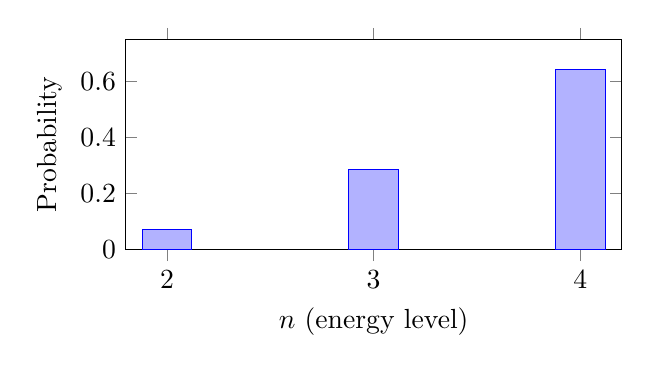
\begin{tikzpicture}
\begin{axis}[
ybar,
bar width=18pt,
xlabel={$n$ (energy level)},
ylabel={Probability},
xtick={2,3,4},
ymin=0, ymax=0.75,
width=0.65\textwidth,
height=0.35\textwidth
]
\addplot coordinates {(2,1/14) (3,4/14) (4,9/14)};
\end{axis}
\end{tikzpicture}
\caption{Energy measurement probabilities.}
\end{figure}

\subsection*{(b) $L^2$: outcomes, probabilities, histogram, and $\langle L^2\rangle$}

For $\ket{n,\ell,m}$,
\[
\hat L^2\ket{n,\ell,m}=\ell(\ell+1)\hbar^2\ket{n,\ell,m}.
\]
The three components have $\ell=1$ (first term) and $\ell=2$ (second and third terms). So
\[
L^2 = 2\hbar^2 \ \ (\ell=1),\qquad
L^2 = 6\hbar^2 \ \ (\ell=2).
\]
Probabilities:
\[
P(L^2=2\hbar^2)=\frac{1}{14},\qquad
P(L^2=6\hbar^2)=\frac{4}{14}+\frac{9}{14}=\frac{13}{14}.
\]
Expectation value:
\[
\langle L^2\rangle
=\frac{1}{14}(2\hbar^2)+\frac{13}{14}(6\hbar^2)
=\frac{40}{7}\hbar^2.
\]
\[
\boxed{\langle L^2\rangle=\frac{40}{7}\hbar^2.}
\]

Histogram (TikZ):
\begin{figure}[H]
\centering
\begin{tikzpicture}
\begin{axis}[
ybar,
bar width=26pt,
xlabel={$L^2$ outcome},
ylabel={Probability},
symbolic x coords={$2\hbar^2$,$6\hbar^2$},
xtick=data,
ymin=0, ymax=1.0,
width=0.65\textwidth,
height=0.35\textwidth
]
\addplot coordinates {($2\hbar^2$,1/14) ($6\hbar^2$,13/14)};
\end{axis}
\end{tikzpicture}
\caption{$L^2$ measurement probabilities.}
\end{figure}

\subsection*{(c) $L_z$: outcomes, probabilities, histogram, and $\langle L_z\rangle$}

For $\ket{n,\ell,m}$,
\[
\hat L_z\ket{n,\ell,m}=m\hbar\ket{n,\ell,m}.
\]
Here the three components have $m=1,-1,2$. So the possible outcomes are
\[
L_z=\hbar,\quad L_z=-\hbar,\quad L_z=2\hbar
\]
with probabilities
\[
P(L_z=\hbar)=\frac{1}{14},\qquad
P(L_z=-\hbar)=\frac{4}{14},\qquad
P(L_z=2\hbar)=\frac{9}{14}.
\]
Expectation value:
\[
\langle L_z\rangle
=\hbar\left[\frac{1}{14}(1)+\frac{4}{14}(-1)+\frac{9}{14}(2)\right]
=\hbar\left(\frac{15}{14}\right).
\]
\[
\boxed{\langle L_z\rangle=\frac{15}{14}\hbar.}
\]

Histogram (TikZ):
\begin{figure}[H]
\centering
\begin{tikzpicture}
\begin{axis}[
ybar,
bar width=18pt,
xlabel={$L_z$ outcome},
ylabel={Probability},
symbolic x coords={$-\hbar$,$\hbar$,$2\hbar$},
xtick=data,
ymin=0, ymax=0.75,
width=0.65\textwidth,
height=0.35\textwidth
]
\addplot coordinates {($-\hbar$,4/14) ($\hbar$,1/14) ($2\hbar$,9/14)};
\end{axis}
\end{tikzpicture}
\caption{$L_z$ measurement probabilities.}
\end{figure}

\subsection*{(d) Time dependence of (a), (b), and (c)}

Time evolution adds phases to each energy eigenstate:
\[
\ket{\psi(t)}
=
\frac{1}{\sqrt{14}}e^{-iE_2 t/\hbar}\ket{2,1,1}
-\frac{2}{\sqrt{14}}e^{-iE_3 t/\hbar}\ket{3,2,-1}
+\frac{3i}{\sqrt{14}}e^{-iE_4 t/\hbar}\ket{4,2,2}.
\]
The magnitudes of the coefficients do not change with time, so the probabilities in
(a), (b), and (c) are time-independent. The expectation values $\langle E\rangle$,
$\langle L^2\rangle$, and $\langle L_z\rangle$ are also time-independent.
\end{document}